\documentclass[a4paper,11pt]{article}

\usepackage[margin=2.5cm]{geometry}
\usepackage{booktabs}
\usepackage{amsmath}
\usepackage{caption}
\usepackage{amssymb}
\usepackage{multirow}
\usepackage{adjustbox}
\usepackage{subcaption}
\usepackage{float}
\usepackage{graphicx}

\begin{document}

\section{Risultati Sperimentali Modal Dropout su DETR}

Le seguenti tabelle riportano i risultati ottenuti sotto diverse configurazioni di \emph{modal dropout} applicate al modello DETR.
Durante l'addestramento, la modalità di input viene campionata in base alle probabilità $P(\text{IR})$, $P(\text{RGB})$ e $P(\text{Fusion})$; in valutazione il modello viene invece testato separatamente sui dataset indicati.

% =========================================================
\subsection{Addestramento su $D_{\text{RGB--IR}}$}

\begin{table}[h]
\centering
\caption{Risultati del modello addestrato su $D_{\text{RGB--IR}}$ con diverse configurazioni di modal dropout.}
\label{tab:rgbir_train}
\begin{tabular}{lcccc}
\toprule
Testato su & $P(\text{IR})$ & $P(\text{RGB})$ & $P(\text{Fusion})$ & mAP@50 \\
\midrule
$D_{\text{IRo}}$ & 100 & 0 & 0 & 0.138 \\
$D_{\text{IRo}}$ & 90 & 0 & 10 & 0.132 \\
$D_{\text{IRo}}$ & 50 & 50 & 0 & 0.163 \\
$D_{\text{IRo}}$ & 37.5 & 37.5 & 25 & 0.132 \\
$D_{\text{IRo}}$ & 25 & 25 & 50 & 0.159 \\
$D_{\text{IRo}}$ & 12.5 & 12.5 & 75 & 0.000 \\
$D_{\text{IRo}}$ & 20 & 20 & 60 & \textbf{0.173} \\
\midrule
$D_{\text{RGB--IR}}$ & 100 & 0 & 0 & 0.379 \\
$D_{\text{RGB--IR}}$ & 90 & 0 & 10 & 0.300 \\
$D_{\text{RGB--IR}}$ & 50 & 50 & 0 & 0.388 \\
$D_{\text{RGB--IR}}$ & 37.5 & 37.5 & 25 & 0.302 \\
$D_{\text{RGB--IR}}$ & 25 & 25 & 50 & 0.377 \\
$D_{\text{RGB--IR}}$ & 12.5 & 12.5 & 75 & 0.000 \\
$D_{\text{RGB--IR}}$ & 20 & 20 & 60 & \textbf{0.417} \\
\bottomrule
\end{tabular}
\end{table}

\newpage
% =========================================================
\subsection{Addestramento su $D_{\text{RGBs--IRa}}$}

\begin{table}[h]
\centering
\caption{Risultati del modello addestrato su $D_{\text{RGBs--IRa}}$ con diverse configurazioni di modal dropout.}
\begin{tabular}{lcccc}
\toprule
Testato su & $P(\text{IR})$ & $P(\text{RGB})$ & $P(\text{Fusion})$ & mAP@50 \\
\midrule
$D_{\text{IRo}}$ & 100 & 0 & 0 & 0.224 \\
$D_{\text{IRo}}$ & 90 & 0 & 10 & 0.261 \\
$D_{\text{IRo}}$ & 50 & 50 & 0 & 0.227 \\
$D_{\text{IRo}}$ & 37.5 & 37.5 & 25 & \textbf{0.306} \\
$D_{\text{IRo}}$ & 25 & 25 & 50 & 0.247 \\
$D_{\text{IRo}}$ & 12.5 & 12.5 & 75 & 0.196 \\
$D_{\text{IRo}}$ & 20 & 20 & 60 & 0.200 \\
\midrule
$D_{\text{RGBs--IRa}}$ & 100 & 0 & 0 & 0.224 \\
$D_{\text{RGBs--IRa}}$ & 90 & 0 & 10 & 0.252 \\
$D_{\text{RGBs--IRa}}$ & 50 & 50 & 0 & 0.219 \\
$D_{\text{RGBs--IRa}}$ & 37.5 & 37.5 & 25 & \textbf{0.280} \\
$D_{\text{RGBs--IRa}}$ & 25 & 25 & 50 & 0.233 \\
$D_{\text{RGBs--IRa}}$ & 12.5 & 12.5 & 75 & 0.205 \\
$D_{\text{RGBs--IRa}}$ & 20 & 20 & 60 & 0.220 \\
\bottomrule
\end{tabular}
\end{table}

% =========================================================
\subsection{Addestramento su $D$}

\begin{table}[h]
\centering
\caption{Risultati del modello addestrato su $D$ con diverse configurazioni di modal dropout.}
\label{tab:all_train}
\begin{tabular}{lcccc}
\toprule
Testato su & $P(\text{IR})$ & $P(\text{RGB})$ & $P(\text{Fusion})$ & mAP@50 \\
\midrule
$D_{\text{IRo}}$ & 100 & 0 & 0 & 0.270 \\
$D_{\text{IRo}}$ & 90 & 0 & 10 & \textbf{0.320} \\
$D_{\text{IRo}}$ & 50 & 50 & 0 & 0.275 \\
$D_{\text{IRo}}$ & 37.5 & 37.5 & 25 & 0.293 \\
$D_{\text{IRo}}$ & 25 & 25 & 50 & 0.270 \\
$D_{\text{IRo}}$ & 12.5 & 12.5 & 75 & 0.158 \\
$D_{\text{IRo}}$ & 20 & 20 & 60 & 0.256 \\
\midrule
$D$ & 100 & 0 & 0 & 0.322 \\
$D$ & 90 & 0 & 10 & \textbf{0.361} \\
$D$ & 50 & 50 & 0 & 0.331 \\
$D$ & 37.5 & 37.5 & 25 & 0.333 \\
$D$ & 25 & 25 & 50 & 0.325 \\
$D$ & 12.5 & 12.5 & 75 & 0.286 \\
$D$ & 20 & 20 & 60 & 0.323 \\
\bottomrule
\end{tabular}
\end{table}

% =========================================================
\begin{table}[h]
\centering

\caption{Confronto diretto tra i risultati originali e i migliori risultati ottenuti con Modal Dropout. Le righe sono raggruppate per set di addestramento e test per evidenziare l'impatto della nuova metodologia.}
\label{tab:summary_comparison}
\begin{tabular}{l c c c c c}
\toprule
\textbf{Trainato su} & \textbf{Testato su} & $\boldsymbol{P(\text{IR})}$ & $\boldsymbol{P(\text{RGB})}$ & $\boldsymbol{P(\text{Fusion})}$ & \textbf{mAP@50} \\
\midrule

% BLOCCO 1: Train su D (Dataset Completo)
\multirow{4}{*}{$D$} 
 & $D$ & 0 & 0 & 100 & \textbf{0.372} \\
 & $D$ & 90 & 0 & 10 & 0.361 \\
 \cmidrule(l){2-6} 
 & $D_{\text{IRo}}$ & 0 & 0 & 100 & 0.233 \\
 & $D_{\text{IRo}}$ & 90 & 0 & 10 & \textbf{0.320} \\
\midrule

% BLOCCO 2: Train su RGB-IR
\multirow{2}{*}{$D_{\text{RGB--IR}}$} 
 & $D_{\text{IRo}}$ & 0 & 0 & 100 & 0.000 \\
 & $D_{\text{IRo}}$ & 20 & 20 & 60 & \textbf{0.173} \\
\midrule

% BLOCCO 3: Train su RGB-IR
\multirow{2}{*}{$D_{\text{RGBs--IRa}}$} 
 & $D_{\text{IRo}}$ & 0 & 0 & 100 & 0.000 \\
 & $D_{\text{IRo}}$ & 37.5 & 37.5 & 25 & \textbf{0.306} \\

\bottomrule
\end{tabular}
\end{table}


% =========================================================
\newpage
\section{Evoluzione con RT-DETR (Real-Time DETR)}

In questa fase della ricerca, l'obiettivo è stato adattare la logica multimodale su un'architettura \textbf{RT-DETR}, ottimizzata per l'inferenza real-time. Sono state testate due strategie principali per gestire la natura multi-scala del modello e la risoluzione ridotta dei target.

\subsection{RT-DETR con Additive Feature Fusion}
Questa architettura utilizza una \textbf{doppia backbone} (ResNet-50vd) 
per elaborare separatamente le modalità RGB e IR. Le \emph{feature maps} 
multi-scala estratte ($P3, P4, P5$) vengono fuse tramite 
\textbf{somma elemento per elemento} (Additive Fusion) e successivamente 
processate dall'\emph{Hybrid Encoder} (AIFI e CCFM). 

Questa scelta presenta due vantaggi chiave: 
\begin{enumerate}
    \item preserva la geometria delle griglie di feature, senza introdurre ulteriori trasformazioni spaziali prima del decoder; 
    \item non introduce parametri addizionali, evitando instabilità 
        durante il \emph{fine-tuning} del modello pre-addestrato su ImageNet.
\end{enumerate}

Il modello è stato addestrato per 10 e 25 epoche utilizzando una strategia 
di \emph{modal dropout} (20\% IR-only, 20\% RGB-only, 60\% fusion - rivelatasi la migliore durante i test sul modello DETR)
per migliorare la robustezza delle modalità singole.

\begin{table}[h]
\centering
\caption{Risultati RT-DETR (Fusion) trainato per 25 epoche su immagine integrale al variare della soglia di confidenza.}
\label{tab:rtdetr_base_25}
\begin{tabular}{lcccc}
\toprule
Testato su & Threshold & mAP@50 (RT-DETR) & mAP@50 (DETR) \\
\midrule
$D_{\text{RGB--IR}}$ & 0.01 & \textbf{0.321} & \multirow{3}{*}{0.417} \\
$D_{\text{RGB--IR}}$ & 0.05 & 0.287 & \\
$D_{\text{RGB--IR}}$ & 0.10 & 0.246 & \\
\midrule
$D_{\text{IRo}}$ & 0.01 & 0.262 & 0.173 \\
$D_{\text{VISo}}$ & 0.01 & 0.264 & - \\
\bottomrule
\end{tabular}
\end{table}

\begin{table}[h]
\centering
\caption{Risultati RT-DETR (Fusion) trainato per 10 epoche su immagine integrale al variare della soglia di confidenza.}
\label{tab:rtdetr_base_10}
\begin{tabular}{lcccc}
\toprule
Testato su & Threshold & mAP@50 (RT-DETR) & mAP@50 (DETR) \\
\midrule
$D_{\text{RGB--IR}}$ & 0.01 & \textbf{0.357} & \multirow{3}{*}{0.417} \\
$D_{\text{RGB--IR}}$ & 0.05 & 0.357 & \\
$D_{\text{RGB--IR}}$ & 0.10 & 0.356 & \\
\midrule
$D_{\text{IRo}}$ & 0.01 & 0.252 & 0.173 \\
$D_{\text{VISo}}$ & 0.01 & 0.246 & - \\
\bottomrule
\end{tabular}
\end{table}

Da queste tabelle notiamo come il training per 10 epoche abbia dato risultati migliori sul dataset fusion ma peggiori sulle singole modalità (RGB/IR). Un aspetto interessante è che in questo caso anche la confidence del modello sembra essere maggiore visto che non c'è quasi alcun peggioramento di prestazioni tra il test con il threshold più basso (0.01) ed il più alto (0.1).
Inoltre, rispetto a DETR questo nuovo approccio peggiora le prestazioni sul dataset fusion (0.417 vs 0.357) ma migliora notevolmente le prestazioni sulle singole modalità (IR $\approx 0.25$ vs $\approx 0.17$).

\newpage

\subsection{RT-DETR con Strategia di Tiling (SAHI-style)}
Per ovviare alla dimensione ridotta dei soggetti, è stato testato un approccio basato su \textbf{tiling}: l'immagine $640 \times 640$ viene divisa in quadranti $320 \times 320$, raddoppiando la scala relativa degli oggetti. Durante il test, le predizioni sui singoli tile vengono rimappate e aggregate tramite NMS globale.

Durante l'\textbf{addestramento}, durato anche in questo caso 10 e 25 epoche, ogni immagine viene ritagliata in modo casuale su uno dei 4 quadranti, mentre durante il \textbf{test} tutti i quadranti vengono processati e aggregati tramite NMS globale (soglia IoU 0.5).

\begin{table}[h]
\centering
\caption{Confronto della robustezza multimodale: RT-DETR Integrale vs RT-DETR con Tiling.}
\label{tab:rtdetr_comparison_final}
\begin{adjustbox}{center}
\begin{tabular}{lccc}
\toprule
\textbf{Test Dataset} & \textbf{Modello Integrale} & \textbf{Modello Tiling (25 ep.)} & \textbf{Modello Tiling (10 ep.)}\\
& (mAP@50) & (mAP@50) & (mAP@50) \\
\midrule
$D_{\text{RGB--IR}}$ & \textbf{0.321} & 0.302 & 0.151 \\
$D_{\text{IRo}}$ & \textbf{0.262} & 0.133 & 0.105 \\
$D_{\text{VISo}}$ & \textbf{0.264} & 0.082 & 0.050\\
\bottomrule
\end{tabular}
\end{adjustbox}
\par\smallskip
\small *I risultati del modello Tiling si riferiscono all'inferenza con aggregazione dei quadranti. \\
Tutti i valori sono riportati con soglia di confidenza 0.01 per evidenziare il potenziale di localizzazione.
\end{table}


% =========================================================
\subsection{RT-DETR con Framework CMX}
È stata infine testata l'integrazione del framework \textbf{CMX} (Zhang et al. 2023), che introduce due moduli avanzati: il \emph{Cross-Modal Feature Rectification Module} (CM-FRM) per calibrare i sensori e il \emph{Feature Fusion Module} (FFM) basato su \emph{Cross-Attention}. L'obiettivo era verificare se una fusione adattiva potesse gestire meglio i disallineamenti spaziali del dataset.

Il modello è stato addestrato per 25 epoche. I risultati evidenziano una netta degradazione delle prestazioni rispetto alla somma additiva.

\begin{table}[h]
\centering
\caption{Risultati RT-DETR con integrazione CMX (25 epoche).}
\label{tab:rtdetr_cmx}
\begin{tabular}{lcccc}
\toprule
Testato su & Threshold & mAP@50 (CMX) & mAP@50 (Base) \\
\midrule
$D_{\text{RGB--IR}}$ & 0.01 & 0.032 & \textbf{0.321} \\
$D_{\text{RGB--IR}}$ & 0.10 & 0.000 & \textbf{0.246} \\
\midrule
$D_{\text{IRo}}$ & 0.01 & 0.081 & \textbf{0.262} \\
$D_{\text{VISo}}$ & 0.01 & 0.018 & \textbf{0.264} \\
\bottomrule
\end{tabular}
\end{table}

Questi risultati documentano il fallimento della specifica integrazione CMX sul dataset WiSARD. La modalità \emph{Fusion} (0.032) risulta notevolmente inferiore alla modalità \emph{IR-only} (0.081), un comportamento compatibile con interferenza tra le modalità. Il disallineamento RGB--IR, l'assenza di coordinate esplicite nell'attenzione e la maggiore complessità di ottimizzazione su un dataset limitato sono spiegazioni plausibili, ma l'esperimento non permette di isolarne causalmente una sola. La confidenza del modello è inoltre rimasta molto bassa, con prestazioni nulle a soglia 0.1.

\subsection{Il Tentativo Ibrido: FAM + CMX + Positional Encoding}

Dall'analisi dei fallimenti del modello CMX puro, sono emerse tre criticità principali strutturali legate allo specifico dominio SAR (Search And Rescue):
\begin{enumerate}
    \item \textbf{Disallineamento e Parallasse:} Il modulo di rettifica (CM-FRM) di CMX assume che le feature map siano "pixel-perfect". In presenza di disallineamento, usare il valore infrarosso per calibrare il pixel visivo sottostante significa mescolare il target con il rumore di fondo, causando una grave interferenza distruttiva.
    \item \textbf{Perdita di Contesto Spaziale nel FFM:} Il modulo di fusione basato su \textit{Cross-Attention} srotola i token temporaneamente privandoli della cognizione 2D. Senza le posizioni relative, si genera \textit{Ghosting} (l'RGB preleva informazioni termiche da parti casuali ma semanticamente affini o "calde" dell'immagine).
    \item \textbf{Collo di bottiglia su P3:} A causa della complessità quadratica $O(N^2)$ dell'attenzione, al livello P3 (quello a più alta risoluzione, vitale per trovare bersagli minuscoli) è necessario applicare un fallback lineare (bypass). Fondendo mappe disallineate con una semplice concatenazione lineare si distruggono irrimediabilmente i piccoli target.
\end{enumerate}

Per affrontare queste criticità è stata progettata un'\textbf{architettura ibrida} che combina i due approcci esplorati. La pipeline elabora le feature nel seguente ordine: $[RGB, IR] \rightarrow FAM \rightarrow CM\text{-}FRM \rightarrow FFM$. 

In pratica, il FAM trasforma preliminarmente le feature IR rispetto al riferimento RGB; segue la calibrazione incrociata CM-FRM e infine la fusione FFM, integrata con un \textbf{2D Sine Positional Encoding} per conservare informazione spaziale esplicita nell'attenzione.

Il modello è stato addestrato e di seguito sono riportati i risultati finali:

\begin{table}[h]
\centering
\caption{Risultati RT-DETR Architettura Ibrida (FAM + CMX + Pos. Encoding).}
\label{tab:rtdetr_cmx_hybrid}
\begin{tabular}{lccc}
\toprule
Testato su & Threshold & mAP@50 (CMX Ibrido) & mAP@50 (CMX Puro) \\
\midrule
$D_{\text{RGB--IR}}$ & 0.01 & \textbf{0.1447} & 0.032 \\
$D_{\text{RGB--IR}}$ & 0.10 & \textbf{0.0878} & 0.000 \\
\midrule
$D_{\text{IRo}}$ & 0.01 & \textbf{0.0944} & 0.081 \\
$D_{\text{IRo}}$ & 0.10 & \textbf{0.0543} & 0.000 \\
\midrule
$D_{\text{VISo}}$ & 0.01 & \textbf{0.1023} & 0.018 \\
$D_{\text{VISo}}$ & 0.10 & \textbf{0.0607} & 0.000 \\
\bottomrule
\end{tabular}
\end{table}

L'ibrido recupera una parte consistente del collasso del CMX puro: la prestazione multimodale passa da 0.032 a 0.1447 e rimane non nulla anche a soglia 0.10. Resta tuttavia nettamente sotto l'Additive Fusion e la migliore variante RT-DETR con FAM e SSJ. L'esperimento mostra quindi che FAM e positional encoding migliorano questa specifica integrazione CMX, senza renderla competitiva con le soluzioni più semplici sul dataset valutato.

\newpage

\section{Ottimizzazione di RT-DETR: Feature Alignment Module}

L'Additive Fusion di RT-DETR combina direttamente feature RGB e IR definite sulla stessa griglia, ma non corregge il disallineamento geometrico introdotto dalla diversa posizione e ottica dei due sensori. Per affrontare questo limite è stato integrato un \textbf{Feature Alignment Module} (FAM) basato su convoluzioni deformabili, posto tra le due backbone e la fusione additiva.

\subsection{Architettura del FAM}

Per ogni livello della piramide, il FAM concatena le feature RGB e IR e usa una convoluzione $3\times3$ per predire 18 componenti di offset e 9 coefficienti di modulazione, corrispondenti ai nove punti di un kernel deformabile $3\times3$:

\[
[\Delta p,m]=\operatorname{Conv}_{3\times3}
    \bigl(\operatorname{Concat}(F_{\mathrm{RGB}},F_{\mathrm{IR}})\bigr).
\]

Gli offset trasformano esclusivamente la feature IR mediante una DCNv2, mentre la feature RGB resta il riferimento:

\[
F'_{\mathrm{IR}}(p)=
\sum_{k=1}^{9}w_k\,F_{\mathrm{IR}}(p+p_k+\Delta p_k)\,m_k,
\qquad
F_{\mathrm{fused}}=F_{\mathrm{RGB}}+F'_{\mathrm{IR}}.
\]

La convoluzione che predice offset e mask è inizializzata a zero: all'avvio gli offset sono nulli e le mask valgono circa 0.5. Ciò preserva inizialmente la griglia di campionamento, ma non rende il FAM un'identità matematica, poiché la DCNv2 conserva pesi convoluzionali propri.

\subsection{Evoluzione architetturale}

\subsubsection{Modello A: inizializzazione lazy}

Nella prima implementazione i moduli FAM venivano creati al primo \textit{forward}, dopo la costruzione dell'optimizer. I loro parametri non entravano quindi nei gruppi di AdamW e restavano invariati durante il training. La trasformazione applicata al ramo IR era fissa e non addestrata; gli offset iniziali erano nulli, non casuali, ma la DCNv2 non costituiva comunque un'identità. La combinazione di un'elevata mAP in fusione (0.4286) e di una mAP IR-only pari a 0.0054 è compatibile con un utilizzo molto ridotto dell'informazione termica, senza tuttavia dimostrare che il ramo IR fosse ignorato completamente.

\subsubsection{Modello B: inizializzazione eager}

I moduli FAM vengono istanziati nel costruttore e aggiornati fin dalla prima iterazione. La mAP IR-only sale a 0.2629, mentre quella in fusione scende a 0.3960. I risultati sono compatibili con una diversa ripartizione del contributo tra le modalità, ma non ne isolano direttamente il meccanismo causale.

\subsubsection{Modello C: FAM congelato}

Il FAM viene costruito correttamente ma mantenuto congelato. Il gradiente può attraversarlo e aggiornare la backbone IR, che può quindi adattarsi alla trasformazione fissa. La configurazione raggiunge 0.2250 in IR-only e 0.3857 in fusione.

\subsubsection{Modello D: Spatial Dropout}

Uno Spatial Dropout al 40\% viene applicato al ramo IR prima della fusione. La configurazione raggiunge 0.3936 in fusione e 0.2716 su VIS-only. La rimozione di interi canali limita però anche informazione semantica potenzialmente utile.

\subsubsection{Modello E: Stochastic Spatial Jitter}

Lo \textbf{Stochastic Spatial Jitter} (SSJ) aggiunge durante il training rumore gaussiano a media nulla agli offset predetti:

\[
\Delta_{\mathrm{train}}=\Delta_{\mathrm{FAM}}+\varepsilon,
\qquad \varepsilon\sim\mathcal{N}(0,\sigma^2).
\]

In inferenza il rumore viene disattivato. L'obiettivo è evitare una dipendenza rigida da una singola corrispondenza spaziale, senza azzerare direttamente i canali IR. Tra le configurazioni RT-DETR valutate, il Modello E ottiene la migliore mAP in fusione, pari a 0.4381.

\subsubsection{Interazione tra SSJ e modal dropout}

Una run addestrata sempre in fusione, senza modal dropout, raggiunge 0.3890 in fusione e una mAP IR-only praticamente nulla. Nel protocollo RT-DETR, SSJ risulta quindi efficace insieme al modal dropout 20\% IR, 20\% RGB e 60\% fusion, che espone esplicitamente il modello anche alle modalità singole. Il risultato positivo osservato su RT-DETR non implica tuttavia che SSJ sia vantaggioso su ogni architettura.

\subsection{Confronto tra le configurazioni}

\begin{table}[htbp]
\centering
\caption{Evoluzione architetturale del FAM e impatto dello Spatial Jitter (mAP@50).}
\label{tab:rtdetr_fam_archit}
\begin{adjustbox}{max width=\textwidth}
\begin{tabular}{lc|ccccc}
\toprule
\textbf{Dataset} & \textbf{Thr} & \textbf{Modello A} & \textbf{Modello B} &
\textbf{Modello C} & \textbf{Modello D} & \textbf{Modello E} \\
& & (Lazy) & (Eager) & (Freeze) & (Spatial Dropout) & (SSJ) \\
\midrule
\multirow{2}{*}{$D_{\text{RGB--IR}}$} & 0.01 & 0.4286 & 0.3960 & 0.3857 & 0.3936 & \textbf{0.4381} \\
& 0.10 & 0.4277 & 0.3944 & 0.3840 & 0.3774 & \textbf{0.4363} \\
\midrule
\multirow{2}{*}{$D_{\text{IRo}}$} & 0.01 & 0.0054 & \textbf{0.2629} & 0.2250 & 0.2248 & 0.1818 \\
& 0.10 & 0.0044 & \textbf{0.2627} & 0.2206 & 0.2167 & 0.1780 \\
\midrule
\multirow{2}{*}{$D_{\text{VISo}}$} & 0.01 & \textbf{0.3000} & 0.2620 & 0.2517 & 0.2716 & 0.2697 \\
& 0.10 & \textbf{0.2987} & 0.2613 & 0.2515 & 0.2674 & 0.2695 \\
\bottomrule
\end{tabular}
\end{adjustbox}
\end{table}

\subsection{Verifica diretta dell'allineamento appreso}

La mAP costituisce un'evidenza indiretta dell'utilità del FAM, ma non dimostra da sola che il modulo apprenda una trasformazione geometrica. È stato quindi sviluppato uno script di diagnostica che registra mediante \textit{forward hook} le feature RGB, IR e FAM(IR), oltre agli offset e alle mask interne. Le feature vengono visualizzate tramite una PCA condivisa a tre componenti, mentre gli offset sono aggregati separatamente per i livelli P3, P4 e P5.

Il confronto principale considera il Modello B, con FAM senza SSJ, e il Modello E, addestrato con FAM e SSJ. Per ciascun checkpoint sono stati analizzati 10 campioni del test set MtErie e 10 campioni per ognuna delle sessioni FHL 210924 e Baker 220109, per un totale di 30 campioni. Le due sessioni aggiuntive appartengono al train split: non misurano la generalizzazione, ma verificano se il campo di offset cambi al variare delle condizioni di acquisizione.

\begin{table}[H]
\centering
\caption{Statistiche degli offset FAM sul test set MtErie, aggregati su dieci campioni e riportati in pixel dell'input al modello. In ciascuna colonna l'ordine è: media / mediana / 90-esimo percentile / massimo.}
\label{tab:fam_alignment_offsets}
\begin{adjustbox}{max width=\textwidth}
\begin{tabular}{cccc}
\toprule
\textbf{Livello} & \textbf{Stride} & \textbf{Offset FAM, B [px]} & \textbf{Offset FAM, E [px]} \\
\midrule
P3 & 8  & 2.74 / 2.50 / 5.17 / 23.07 & 4.01 / 3.08 / 9.13 / 30.51 \\
P4 & 16 & 2.66 / 2.02 / 5.69 / 59.23 & 4.18 / 3.23 / 9.27 / 56.57 \\
P5 & 32 & 3.95 / 3.10 / 7.87 / 94.08 & 4.61 / 3.79 / 8.47 / 204.54 \\
\bottomrule
\end{tabular}
\end{adjustbox}
\end{table}

\begin{table}[H]
\centering
\caption{Controllo cross-sessione degli offset FAM. Le sessioni FHL 210924 e Baker 220109 appartengono al train split; per ogni riga sono aggregati dieci campioni. In ciascuna cella l'ordine è: media / mediana / 90-esimo percentile, in pixel dell'input al modello.}
\label{tab:fam_alignment_cross_session}
\begin{adjustbox}{max width=\textwidth}
\begin{tabular}{cccc}
\toprule
\textbf{Modello / sessione} & \textbf{Offset P3 [px]} & \textbf{Offset P4 [px]} & \textbf{Offset P5 [px]} \\
\midrule
B -- FHL 210924   & 2.57 / 2.24 / 4.89 & 2.63 / 1.97 / 5.66 & 3.81 / 2.92 / 7.64 \\
B -- Baker 220109 & 2.33 / 1.88 / 4.68 & 2.67 / 2.01 / 5.78 & 4.03 / 3.17 / 7.95 \\
E -- FHL 210924   & 3.75 / 2.89 / 8.45 & 4.11 / 3.09 / 9.26 & 4.60 / 3.78 / 8.56 \\
E -- Baker 220109 & 3.30 / 2.65 / 6.97 & 4.02 / 2.90 / 9.27 & 4.68 / 3.68 / 9.02 \\
\bottomrule
\end{tabular}
\end{adjustbox}
\end{table}

Gli offset tipici sono dell'ordine di pochi pixel e risultano non nulli in entrambi i modelli. Il Modello E presenta medie e mediane maggiori a tutti i livelli. A P3 e P4 SSJ produce inoltre campi mediamente più uniformi nello spazio; a P5 l'effetto non è stabile e compaiono massimi isolati molto elevati, mentre il 90-esimo percentile resta inferiore a 10 pixel.

Il controllo sulle sessioni FHL e Baker conserva lo stesso ordine di grandezza, ma le medie cambiano di circa 2--12\% tra sessioni. Il FAM non è quindi riconducibile a un unico offset globale fisso comune alle tre acquisizioni: l'evidenza è compatibile con una correzione condizionata dall'input e dalle condizioni geometriche della sessione, con una possibile componente stabile legata alla configurazione dei sensori. Le statistiche aggregate non separano tuttavia una dipendenza dalla singola immagine da una dipendenza dalla sessione; per misurare direttamente quanto cambino i campi cella per cella saranno necessari confronti tra tensori, ad esempio tramite MAE o correlazione.

Le feature FAM(IR) appaiono inoltre più lisce delle feature IR iniziali. Questo comportamento è compatibile con lo smoothing introdotto dal campionamento bilineare e dalla combinazione modulata dei nove punti della DCNv2; non deve essere interpretato automaticamente come un miglioramento o un collasso semantico.

\subsection{Analisi qualitativa delle predizioni IR-only}

Nonostante la differenza di mAP@50 tra il Modello A (0.0044) e il Modello E (0.1780), le predizioni mostrano strategie operative differenti. Nelle immagini con segnale termico debole il Modello A tende a non produrre detection, mentre il Modello E aumenta la copertura al costo di più falsi positivi. Quando il segnale è netto, il Modello A può invece produrre poche predizioni con confidenza relativamente maggiore.

\begin{figure}[H]
    \centering
    \begin{subfigure}[t]{0.45\textwidth}
        \centering
        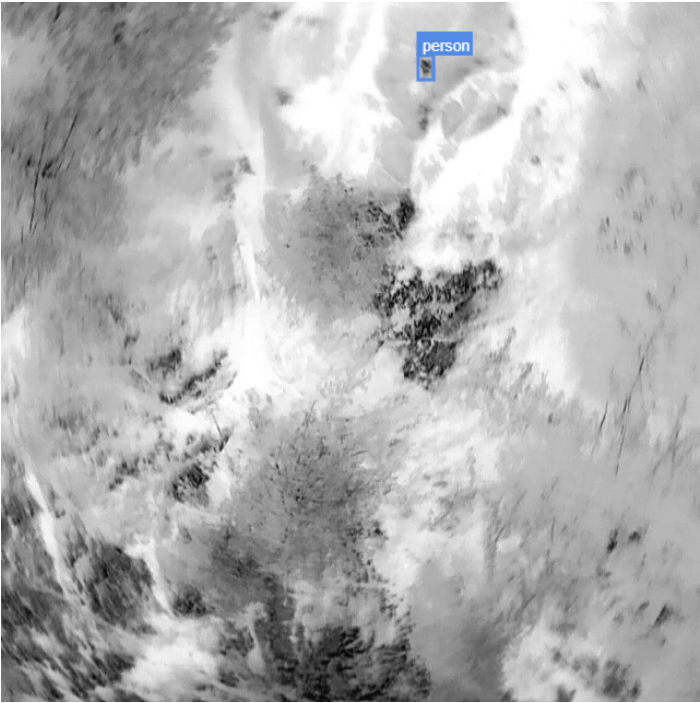
\includegraphics[width=\textwidth]{images/modA_weak_signal.png}
        \caption{Modello A: nessuna predizione generata.}
    \end{subfigure}
    \hfill
    \begin{subfigure}[t]{0.45\textwidth}
        \centering
        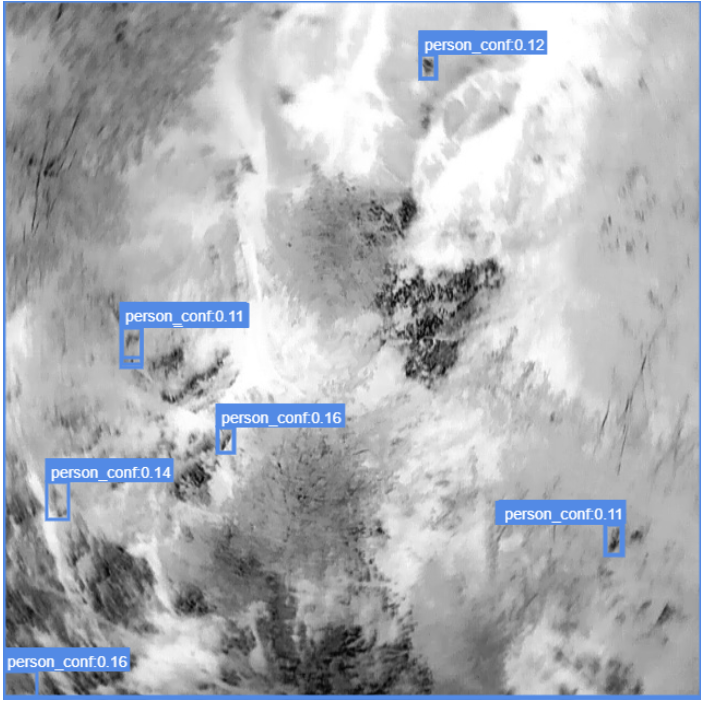
\includegraphics[width=\textwidth]{images/modE_weak_signal.png}
        \caption{Modello E: target corretto tra diversi falsi positivi.}
    \end{subfigure}
    \caption{Confronto su un'immagine IR con segnale termico debole.}
    \label{fig:qualitative_weak}
\end{figure}

\begin{figure}[H]
    \centering
    \begin{subfigure}[t]{0.45\textwidth}
        \centering
        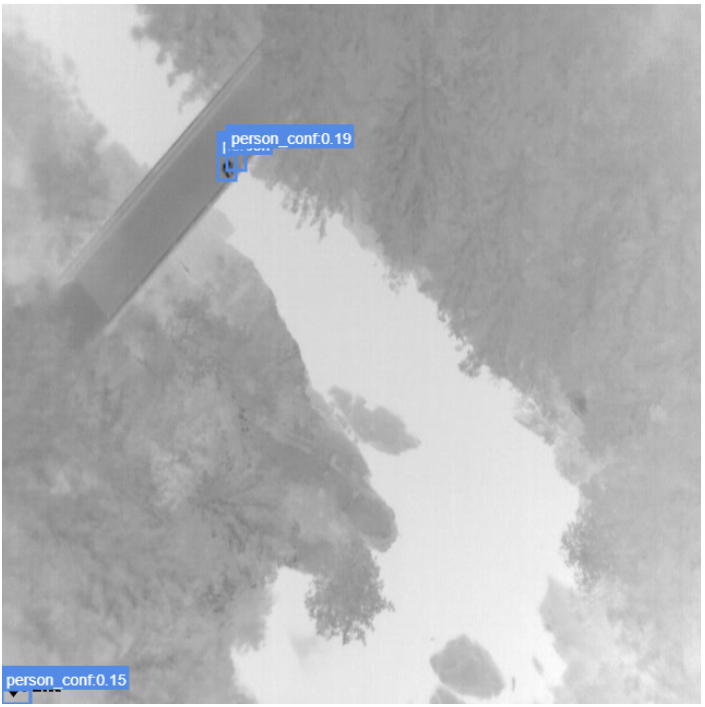
\includegraphics[width=\textwidth]{images/modA_strong_signal.png}
        \caption{Modello A: target corretto con confidenza 0.19.}
    \end{subfigure}
    \hfill
    \begin{subfigure}[t]{0.45\textwidth}
        \centering
        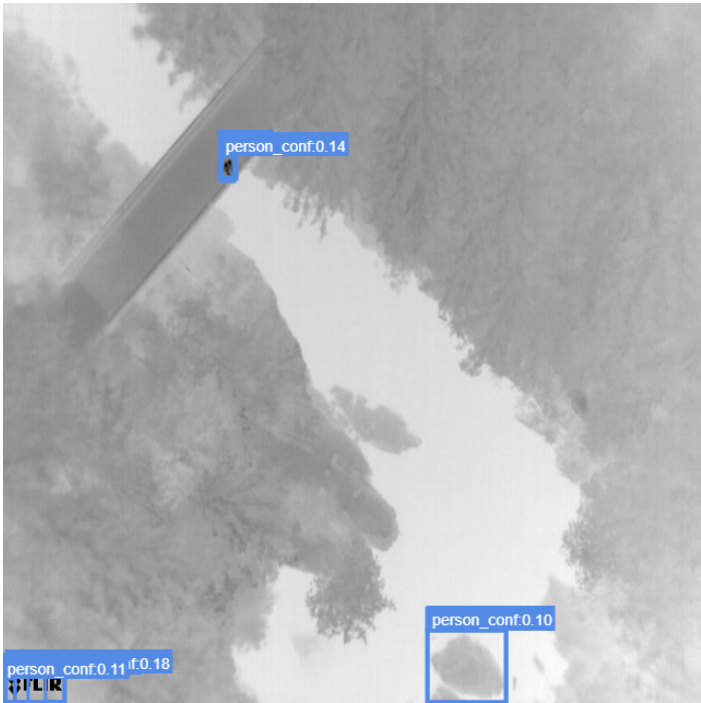
\includegraphics[width=\textwidth]{images/modE_strong_signal.png}
        \caption{Modello E: target con confidenza 0.14 e un falso positivo.}
    \end{subfigure}
    \caption{Confronto su un'immagine IR con segnale termico netto.}
    \label{fig:qualitative_strong}
\end{figure}

Su circa il 38\% delle immagini IR-only il Modello A non genera predizioni. Il comportamento è compatibile con un detector più conservativo, ma le osservazioni qualitative non sono sufficienti per attribuirlo unicamente al bug di inizializzazione né per stabilire che sia preferibile in un impiego operativo: in uno scenario SAR il costo dei falsi negativi deve essere valutato insieme a quello dei falsi allarmi.

\newpage

\section{Evoluzione con Deformable DETR: Dalla Fusione Spaziale alla Channel Concatenation}

Successivamente la ricerca si è spostata sull'architettura \textbf{Deformable DETR}. L'obiettivo era sfruttare il meccanismo di attenzione sparsa (Deformable Attention) per gestire meglio le feature multi-scala, cercando un compromesso tra la complessità computazionale del CMX e la semplicità della somma additiva.

In questa fase sono stati esplorati due approcci distinti di fusione delle feature, portando allo sviluppo di un'architettura dedicata basata sulla concatenazione dei canali.

\subsection{Il fallimento della Fusione Spaziale (Spatial Concatenation)}
Il primo tentativo di adattamento ha previsto una strategia di \textit{Spatial Concatenation}. In questa configurazione, le feature map provenienti dalla backbone RGB e da quella IR sono state concatenate lungo l'asse dell'altezza (dimensione $H$), raddoppiando di fatto la dimensione verticale del tensore di input per l'encoder ($H_{in} \rightarrow 2H$).

L'ipotesi era che il meccanismo di attenzione deformabile potesse apprendere autonomamente le relazioni tra le due modalità. Tuttavia, l'approccio ha presentato due criticità fatali:
\begin{itemize}
    \item \textbf{Esplosione Computazionale:} Il raddoppio delle dimensioni spaziali ha costretto a ridurre i livelli delle feature map (da 4 a 2) per evitare problemi di memoria (OOM), limitando la capacità del modello di rilevare oggetti a diverse scale.
    \item \textbf{Rottura Semantica:} Alterare la geometria spaziale invalida i \textit{reference points} pre-addestrati, introducendo una discontinuità che il modello non è riuscito a compensare, portando a metriche mAP prossime allo zero.
\end{itemize}

\subsection{Implementazione della Channel Concatenation con Proiezione}
Per preservare l'allineamento spaziale e la capacità rappresentativa originale, è stata implementata una nuova strategia basata sulla \textbf{Channel Concatenation}, definita nel modulo \newline \texttt{DeformableDetrFusionBackbone}.

A differenza dell'approccio precedente, questa architettura mantiene inalterate le dimensioni spaziali ($H \times W$) e opera la fusione lungo la dimensione dei canali. Il processo si articola nei seguenti step:

\begin{enumerate}
    \item \textbf{Dual Backbone Indipendente:} Vengono istanziate due backbone parallele (ResNet-50) per estrarre le feature separatamente da RGB e IR. I pesi della backbone IR sono inizializzati adattando quelli pre-addestrati su RGB (media dei canali) per favorire la convergenza.
    \item \textbf{Concatenazione e Fusione Non Lineare:} Per ogni livello della piramide di feature, le feature $F_{RGB}$ e $F_{IR}$ vengono inizialmente concatenate lungo la dimensione dei canali ($2C_i$). Invece di una semplice proiezione lineare, viene applicato un blocco di fusione più strutturato composto da:
    \begin{itemize}
        \item \textbf{Convoluzione 1x1:} Riduce i canali da $2C_i$ a $C_i$, operando una prima miscelazione delle informazioni.
        \item \textbf{Group Normalization:} Stabilizza l'output (32 gruppi), garantendo robustezza statistica anche con \textit{batch size} molto ridotti (\texttt{batch\_size=1} nella configurazione adottata).
        \item \textbf{Activation (ReLU):} Introduce non-linearità, permettendo al blocco di modulare il contributo di ciascuna modalità in funzione del segnale piuttosto che limitarsi a una combinazione lineare fissa.
    \end{itemize}
    $$ F_{fused} = \text{ReLU}\big(\text{GN}(\text{Conv}_{1\times1}(\text{Concat}(F_{RGB}, F_{IR})))\big) $$
    Questo blocco di fusione è condiviso dalle configurazioni baseline, FAM e FAM + SSJ e dalla successiva architettura DINO.
    \item \textbf{Mantenimento della Multi-Scala:} Le due backbone producono tre livelli nativi. Dopo la fusione, Deformable DETR genera un quarto livello a risoluzione inferiore applicando una convoluzione $3\times3$ con stride 2 alla C5 fusa. Il quarto livello non deriva quindi da una quarta coppia RGB--IR e non attraversa un ulteriore FAM.
\end{enumerate}

Le feature vengono proiettate a $d_{\mathrm{model}}=256$, appiattite e concatenate nella sequenza fornita all'encoder. Il processor di \texttt{SenseTime/deformable-detr} ridimensiona preservando l'aspect ratio, con lato corto fino a 800 pixel e lato lungo fino a 1333; il numero di token varia quindi con la forma dell'immagine preprocessata. Per un input effettivamente quadrato $800\times800$, i quattro livelli misurano $100\times100$, $50\times50$, $25\times25$ e $13\times13$, per un totale di 13294 token.

Le feature ottenute vengono passate all'encoder insieme alle codifiche posizionali. Il decoder usa 300 query apprendibili e alterna self-attention tra le query e cross-attention deformabile multi-scala verso le feature dell'encoder. Ciascuna query produce infine una classificazione e un bounding box.

Questa configurazione preserva la geometria e il numero di livelli attesi dal checkpoint pretrained. La fusione di canale evita di alterare artificialmente gli assi spaziali, pur lasciando al FAM opzionale il compito di compensare il disallineamento residuo tra i sensori.

\subsection{Integrazione del modulo FAM e SSJ}
A seguito dei risultati ottenuti su RT-DETR, lo stesso schema di allineamento è stato integrato nella backbone di fusione di Deformable DETR. Il FAM opera sui tre livelli nativi prima della concatenazione di canale. I pesi di \texttt{offset\_conv} sono inizializzati a zero, per cui gli offset iniziali sono nulli e la geometria di campionamento parte non deformata; la DCNv2 mantiene però pesi propri e il modulo complessivo non è un'identità.

Lo \textbf{Stochastic Spatial Jitter} aggiunge esclusivamente durante il training rumore gaussiano agli offset predetti, prima della DCNv2. L'obiettivo è regolarizzare il campo di allineamento rispetto a piccole perturbazioni; il suo effetto deve però essere verificato separatamente per ciascuna architettura.

\subsection{Instabilità Run-to-Run dell'Attenzione Deformabile}
\label{sec:instabilita_deformable}

Durante la campagna sperimentale su questa famiglia di modelli è emerso un fenomeno non osservato con RT-DETR: a parità di seed, esecuzioni successive del medesimo addestramento producono risultati finali significativamente diversi (variazioni di mAP@50 anche superiori a 0.10). Poiché ogni sorgente di stocasticità controllata dal seed (ordine di shuffling del DataLoader, scelta della modalità in \texttt{modal\_dropout}) è deterministica a parità di seed, questa osservazione esclude di per sé tali fattori come causa: la sorgente di non-determinismo risiede altrove.

La causa è stata identificata nel kernel CUDA che implementa la \textit{Multi-Scale Deformable Attention}. Il passo all'indietro (\textit{backward}) di questo kernel deve retro-propagare il gradiente verso le posizioni campionate (non intere) della feature map; poiché più query possono campionare la stessa cella o celle adiacenti, l'accumulo richiede operazioni \texttt{atomicAdd}. L'ordine con cui i thread eseguono questi accumuli non è deterministico, e poiché la somma in virgola mobile non è associativa, l'esito numerico del backward cambia leggermente a ogni esecuzione, anche a parità di seed e di dato in ingresso. RT-DETR, basato su attenzione standard \textit{scaled dot-product}, ha un backward interamente deterministico: questo spiega perché la stessa instabilità non sia mai stata osservata in quell'architettura.

Una piccola perturbazione numerica nel gradiente non spiegherebbe, da sola, oscillazioni di 0.10 mAP: l'amplificazione avviene tramite il matcher di Hungarian, che assegna in modo discreto ogni query alle ground truth disponibili. Tale assegnazione è una funzione discontinua dei logit e delle box predette: una minima divergenza numerica può alterare l'assegnazione già nelle prime iterazioni, portando le query a specializzarsi su oggetti diversi in esecuzioni diverse e le rispettive traiettorie di addestramento a divergere in modo permanente.

Si è inoltre verificato che \texttt{torch.use\_deterministic\_algorithms(True)} non costituisce una soluzione praticabile: il kernel di Deformable Attention non possiede un'implementazione CUDA deterministica, per cui l'attivazione del flag forza un fallback estremamente lento (epoche da oltre 4 ore contro i $\sim$35--40 minuti tipici), rendendo l'addestramento deterministico non sostenibile su questo dataset.

Di conseguenza, le tre configurazioni Deformable DETR sono state eseguite su cinque seed e vengono riportate come \textbf{mediana e intervallo minimo--massimo}. Lo stesso protocollo è stato adottato per la campagna DINO completa base. La run con seed 42 è stata esclusa a causa di un tempo per epoca anomalo ($\sim$2h contro $\sim$35$--$40 minuti).

Un'analisi di potenza statistica conferma che $n=5$ non è sufficiente a distinguere le configurazioni Deformable DETR: per confermare con potenza dell'80\% ($\alpha=0.05$) il guadagno medio osservato per FAM sarebbero necessarie circa 48 run per configurazione; usando il guadagno sulla mediana, la stima più favorevole è di circa 13 run. FAM mostra la tendenza più promettente, ma gli intervalli restano ampiamente sovrapposti.

\subsection{Risultati su Deformable DETR: Baseline, FAM e FAM + SSJ}

La Tabella~\ref{tab:def_detr_results} riporta mediana e range su 5 seed per le tre configurazioni testate, a soglia di confidenza 0.01.

\begin{table}[h]
\centering
\caption{Risultati Deformable DETR (Fusion), confidence threshold 0.01. Per le configurazioni basate su Deformable DETR i valori sono mediana [range] su 5 run con seed differenti; per RT-DETR e DETR (attenzione standard, deterministica) si riportano i valori a singola run.}
\label{tab:def_detr_results}
\begin{adjustbox}{max width=\textwidth}
\begin{tabular}{lccc}
\toprule
Configurazione & $D_{\text{VISo}}$ & $D_{\text{IRo}}$ & $D_{\text{RGB--IR}}$ \\
\midrule
Deformable DETR (baseline) & 0.157~[0.131--0.197] & 0.115~[0.086--0.142] & 0.249~[0.199--0.303] \\
\quad + FAM & 0.184~[0.171--0.253] & 0.131~[0.097--0.165] & 0.294~[0.213--0.314] \\
\quad + FAM + SSJ & 0.142~[0.115--0.206] & 0.088~[0.073--0.109] & 0.263~[0.170--0.350] \\
\midrule
RT-DETR (singola run) & 0.246 & 0.252 & 0.357 \\
DETR (singola run) & -- & 0.173 & 0.417 \\
\bottomrule
\end{tabular}
\end{adjustbox}
\end{table}

Il modulo FAM è l'unica variante che mostra una separazione visibile sulla mediana rispetto alla baseline (0.294 contro 0.249 in $D_{\text{RGB--IR}}$), sebbene il range superiore della baseline (0.303) si sovrapponga ampiamente al range del FAM. Lo Stochastic Spatial Jitter, che in RT-DETR aveva un effetto stabilizzante, produce qui l'effetto opposto: il range di FAM + SSJ (0.170--0.350) è il più ampio delle tre configurazioni, quasi il doppio di baseline e FAM. Una possibile spiegazione è che il rumore spaziale iniettato dallo SSJ interagisca con il non-determinismo del kernel di Deformable Attention descritto in \S\ref{sec:instabilita_deformable}, sommando due sorgenti di varianza indipendenti invece di compensarne una con l'altra come accade con l'attenzione standard di RT-DETR.

In nessun caso i tre intervalli risultano statisticamente separabili al numero di seed attuale; anche il confronto con il singolo valore disponibile per RT-DETR (0.357) o DETR (0.417) va quindi letto come indicativo, non come una differenza consolidata.

\newpage

\section{Integrazione di DINO (DETR with Improved DeNoising Anchor Boxes)}

DINO mantiene la dual backbone, il FAM opzionale e la Channel Fusion descritti per Deformable DETR, ma converte il detector in una configurazione two-stage con box refinement attivo. L'implementazione comprende le tre componenti principali di DINO: \textit{Mixed Query Selection} (MQS), \textit{Contrastive DeNoising} (CDN) e \textit{Look-Forward-Twice} (LFT).

\subsection{Mixed Query Selection}

L'encoder assegna classe e bounding box alle proposal spaziali e seleziona le 300 con score di foreground più elevato. MQS separa il ruolo geometrico dal contenuto delle query:

\begin{itemize}
    \item le proposal dell'encoder forniscono gli anchor e le codifiche posizionali iniziali;
    \item il contenuto delle query proviene da un embedding appreso, inizializzato tramite le query pretrained di Deformable DETR.
\end{itemize}

In inferenza il decoder riceve soltanto queste 300 matching query. Gli anchor sono quindi condizionati all'immagine, mentre il contenuto conserva un warm start compatibile con il checkpoint one-stage.

\subsection{Contrastive DeNoising (CDN)}

Durante il training vengono aggiunte query di denoising costruite dalle annotazioni. Con $M$ ground truth massime nel batch e $G$ gruppi, il numero di query CDN è $2GM$; nella configurazione corrente $G=5$. Per ogni gruppo vengono prodotte copie positive e negative:

\begin{itemize}
    \item label e bounding box in ingresso vengono perturbati in modo controllato;
    \item le copie positive ricostruiscono classe e box originali;
    \item le copie negative sono supervisionate come background nel solo ramo di classificazione e non ricevono loss L1 o GIoU.
\end{itemize}

Una maschera additiva impedisce alle matching query di leggere le query CDN e separa i diversi gruppi di denoising. La self-attention del decoder consuma effettivamente questa maschera. La loss ausiliaria comprende focal loss di classificazione, L1 e GIoU, viene applicata a ogni decoder layer ed è normalizzata rispetto al numero di copie positive. Gli slot CDN sono rimossi prima delle predizioni standard e non vengono creati in inferenza.

\subsection{Look-Forward-Twice}

Il decoder raffina iterativamente i bounding box a ogni layer. LFT mantiene due versioni del nuovo reference point: una copia \texttt{detach()} viene passata alla deformable attention del layer successivo, mentre la copia non detached viene conservata per calcolare la predizione successiva. In questo modo la loss del layer seguente può aggiornare anche la testa box del layer precedente senza retropropagare attraverso l'intera catena delle operazioni di attenzione.

Il refinement è attivo esplicitamente tramite \texttt{with\_box\_refine=True}. La positional query viene rigenerata dall'anchor raffinato prima di ciascun decoder layer.

\subsection{Inizializzazione dal checkpoint}

Il modello parte da \texttt{SenseTime/deformable-detr}. Le componenti compatibili mantengono i pesi pretrained: backbone RGB, backbone IR adattata mediando i canali della prima convoluzione, encoder, decoder e layer interni delle teste box. Il contenuto MQS riceve un warm start dalle query pretrained e la trasformazione dell'output encoder viene inizializzata come identità. Gli output layer delle teste di raffinamento partono da zero, così ogni layer aggiorna l'anchor corrente senza introdurre un delta casuale incompatibile.

Alle teste di classificazione del decoder e dell'encoder viene applicato il prior DINO di foreground all'1\%, evitando che una probabilità iniziale eccessiva domini la focal loss. Channel Fusion, FAM, embedding CDN e trasformazioni two-stage vengono invece appresi durante i nuovi training con learning rate dedicato.

\subsection{Risultati e decisione sperimentale}

Il DINO completo base è stato eseguito su cinque seed; il risultato è espresso come mediana e intervallo minimo--massimo del test mAP@50, a soglia di confidenza 0.01.

\begin{table}[htbp]
\centering
\caption{Risultati della campagna DINO completa base, a soglia di confidenza 0.01. I valori sono mediana [min--max] su cinque seed.}
\label{tab:dino_status}
\begin{tabular}{lccc}
\toprule
Configurazione & $D_{\text{IRo}}$ & $D_{\text{VISo}}$ & $D_{\text{RGB--IR}}$ \\
\midrule
DINO completo & 0.0565 [0.0232--0.1091] & 0.0881 [0.0671--0.1473] & 0.1088 [0.0669--0.1635] \\
\bottomrule
\end{tabular}
\end{table}

La mediana in fusione è pari a 0.1088 e anche il miglior seed (0.1635) resta inferiore alla mediana del Deformable DETR base (0.249). Lo stesso scarto è presente nelle modalità singole. Alla luce di questi risultati, le campagne DINO + FAM e DINO + FAM + SSJ non vengono avviate: senza una nuova ipotesi di ottimizzazione o implementazione, il loro costo sperimentale non è giustificato da una base così debole. Il risultato non implica che DINO sia intrinsecamente inadatto al problema, ma circoscrive la decisione alla configurazione e al budget di training valutati.

\newpage

\section{YOLOv10 con dual backbone e FAM}

Per verificare la trasferibilità del metodo a un detector convoluzionale è stata sviluppata una variante fusion di YOLOv10s. Il modello usa due backbone: una RGB inizializzata dai pesi COCO e una IR il cui primo layer viene adattato da tre a un canale mediante la media dei pesi pretrained. Le feature P3, P4 e P5 delle due backbone vengono elaborate da tre FAM indipendenti e fuse per somma:

\[
F_i=F_{\mathrm{RGB},i}+\operatorname{FAM}_i
\bigl(F_{\mathrm{RGB},i},F_{\mathrm{IR},i}\bigr),
\qquad i\in\{\mathrm{P3},\mathrm{P4},\mathrm{P5}\}.
\]

Le feature già fuse alimentano il neck FPN/PAN e la testa \texttt{v10Detect}. Il task è single-class, con la sola classe persona. La variante senza FAM contiene circa 11.96 milioni di parametri; l'integrazione dei tre moduli FAM porta il totale a circa 15.49 milioni.

\subsection{Risultati fusion-only}

Questa prima campagna è stata addestrata sempre in modalità fusion, senza modal dropout. Le configurazioni senza FAM e con valori SSJ diversi sono funzionalmente identiche, poiché SSJ non viene applicato quando i moduli FAM sono disabilitati; le tre run corrispondenti hanno infatti prodotto file dei risultati identici e sono rappresentate da una sola baseline effettiva.

\begin{table}[htbp]
\centering
\caption{Risultati YOLOv10 single-class. Ogni riga rappresenta una singola run indipendente; il training è stato eseguito esclusivamente in modalità fusion.}
\label{tab:yolo_results}
\begin{tabular}{lccc}
\toprule
Configurazione & $D_{\text{RGB--IR}}$ & $D_{\text{VISo}}$ & $D_{\text{IRo}}$ \\
\midrule
YOLOv10 + FAM, SSJ $=0.0$ & \textbf{0.4074} & 0.1713 & 0 \\
YOLOv10 + FAM, SSJ $=0.5$ & 0.2982 & \textbf{0.1955} & 0 \\
YOLOv10 + FAM, SSJ $=1.0$ & 0.3331 & 0.1538 & $\sim2.8\times10^{-6}$ \\
YOLOv10 senza FAM & 0.3776 & 0.0782 & $\sim3.1\times10^{-8}$ \\
\bottomrule
\end{tabular}
\end{table}

FAM senza SSJ ottiene il miglior risultato fusion della campagna (0.4074), mentre le due configurazioni con jitter restano sotto la baseline senza FAM. Tutte le varianti FAM migliorano invece nettamente la valutazione VIS-only rispetto alla baseline. Poiché è disponibile una sola run per configurazione, questi andamenti sono esplorativi e non consentono di separare l'effetto architetturale dalla variabilità della singola inizializzazione.

La mAP IR-only praticamente nulla è coerente con il protocollo fusion-only: durante il training il modello non è mai stato esposto all'assenza del canale RGB e non ha quindi appreso robustezza alla modalità termica isolata.

\subsection{Modal dropout: input-level e feature gating}

La campagna successiva ha adottato la stessa distribuzione 20\% IR-only, 20\% VIS-only e 60\% fusion già impiegata negli altri detector. Sono state valutate due implementazioni. Nel \emph{modal dropout input-level} la modalità assente viene azzerata nell'immagine, ma entrambe le backbone continuano a essere eseguite. Bias convoluzionali e BatchNorm possono quindi produrre feature non nulle anche dal ramo formalmente assente; inoltre, in IR-only, il FAM tenta di allineare l'IR usando come riferimento feature VIS prive di contenuto reale.

\begin{table}[H]
\centering
\caption{YOLOv10 con modal dropout input-level 20/20/60. Valori mAP@50 sul test set; ogni riga è una singola run.}
\label{tab:yolo_md_input}
\begin{tabular}{lccc}
\toprule
Configurazione & Fusion & VIS-only & IR-only \\
\midrule
YOLOv10 + FAM, SSJ $=0.0$ & 0.329 & 0.158 & \textbf{0.054} \\
YOLOv10 + FAM, SSJ $=0.5$ & \textbf{0.379} & \textbf{0.179} & 0.018 \\
YOLOv10 + FAM, SSJ $=1.0$ & 0.334 & 0.166 & 0.013 \\
YOLOv10 senza FAM & 0.334 & 0.131 & 0.023 \\
\bottomrule
\end{tabular}
\end{table}

L'input-level dropout evita lo zero assoluto in IR-only, ma il massimo ottenuto è 0.054 e non rappresenta una robustezza operativa. Non emerge inoltre un miglioramento sistematico in VIS-only o fusion: il caso FAM con SSJ $=0.5$ migliora rispetto alla propria baseline fusion-only, che era però una configurazione particolarmente debole.

La seconda implementazione introduce invece un \emph{feature gating} esplicito. In VIS-only il neck riceve soltanto le feature VIS; in IR-only riceve soltanto le feature IR e il FAM viene bypassato, poiché non esiste un riferimento VIS reale; in full-fusion rimane invariata la somma tra VIS e IR allineato dal FAM. La strategia è selezionabile nel codice, così da conservare anche il comportamento input-level usato negli esperimenti storici.

\begin{table}[H]
\centering
\caption{YOLOv10 con modal dropout 20/20/60 e feature gating. Valori mAP@50 sul test set; ogni riga è una singola run.}
\label{tab:yolo_md_feature}
\begin{tabular}{lccc}
\toprule
Configurazione & Fusion & VIS-only & IR-only \\
\midrule
YOLOv10 + FAM, SSJ $=0.0$ & 0.2965 & 0.0750 & 0.0356 \\
YOLOv10 + FAM, SSJ $=0.5$ & 0.3335 & 0.1454 & 0.0308 \\
YOLOv10 + FAM, SSJ $=1.0$ & 0.2358 & 0.0638 & 0.0295 \\
YOLOv10 senza FAM & \textbf{0.3469} & \textbf{0.1756} & \textbf{0.0616} \\
\bottomrule
\end{tabular}
\end{table}

Nel regime feature-gated, la variante senza FAM domina tutte le configurazioni FAM nelle tre modalità. Rispetto al corrispondente input-level, migliora fusion da 0.334 a 0.347, VIS-only da 0.131 a 0.176 e IR-only da 0.023 a 0.062. Ciò conferma l'utilità strutturale di escludere realmente il ramo assente, ma il risultato IR-only rimane molto inferiore all'intervallo circa 0.18--0.26 osservato nelle varianti RT-DETR con FAM. Il modal dropout 20/20/60 non trasferisce quindi automaticamente a YOLO la robustezza ottenuta con RT-DETR.

Questa campagna mostra inoltre che il contributo del FAM dipende dall'architettura e dal regime di training. Su YOLO fusion-only, FAM senza SSJ migliora la baseline (0.407 contro 0.378), ma il vantaggio non è universale: con feature gating tutte le varianti FAM sono inferiori alla baseline senza FAM. Le singole run disponibili non consentono comunque di separare completamente l'effetto architetturale dalla variabilità di inizializzazione.

\subsection{Diagnostica preliminare del FAM}

La diagnostica interna è stata applicata ai tre checkpoint YOLO con FAM su tre campioni del validation set. Gli offset medi aumentano scendendo da P3 a P5 e, nel checkpoint migliore senza SSJ, valgono rispettivamente 9.5, 21.9 e 42.7 pixel dell'input. A P5 la deviazione standard spaziale di FAM(IR) risulta 4.5 volte inferiore a quella della feature IR iniziale; il rapporto sale a 6.3 e 20.1 nelle due configurazioni con SSJ.

Questi risultati mostrano che il FAM è attivo, ma il campione è troppo ridotto per un confronto quantitativo con RT-DETR. Un'estensione rigorosa richiederebbe gli stessi 30 campioni distribuiti tra MtErie, FHL e Baker e offset normalizzati rispetto alla risoluzione, poiché YOLO e RT-DETR usano preprocessing differenti.

\subsection{Validation set e selezione del checkpoint}

Una valutazione standalone del checkpoint feature-gated senza FAM sullo split di validazione ha restituito mAP50--95 pari a 0.00353 e mAP@50 pari a 0.01563, coerenti con i valori registrati durante il training. La bassa validation mAP non deriva quindi da un errore specifico del validator YOLO. Anche RT-DETR e Deformable DETR mostrano valori bassi sul medesimo split, indicando una limitazione del protocollo condiviso e non una fragilità esclusiva di YOLO.

Dopo il filtro delle sequenze prive di annotazioni, la validation RGB--IR effettiva contiene infatti una sola sessione FHL: 273 immagini, di cui 184 background, e 148 bounding box complessive. Il test set comprende invece tre sequenze MtErie. Lo split di validazione è pertanto piccolo, sbilanciato verso i background, limitato a una singola sessione e non rappresentativo della varietà del test. Questa composizione costituisce una spiegazione plausibile delle metriche basse osservate trasversalmente, pur non isolandone da sola tutto il contributo.

La selezione resta inoltre leggermente diversa tra famiglie: YOLO salva \texttt{best.pt} ed esegue l'early stopping sulla fitness
\[
0.1\,\mathrm{mAP@50}+0.9\,\mathrm{mAP@50\text{--}95},
\]
calcolata soltanto sulla modalità fusion, mentre RT-DETR e Deformable DETR monitorano direttamente la mAP50--95. Le prestazioni VIS-only e IR-only non partecipano quindi alla scelta del checkpoint YOLO. Il confronto sul test comune rimane internamente coerente, ma la selezione dell'epoca migliore può essere rumorosa e poco rappresentativa per tutti i modelli. Un eventuale validation set revisionato dovrebbe essere applicato coerentemente almeno ai modelli principali e mantenuto rigorosamente separato dal test; modificarlo soltanto per YOLO comprometterebbe la comparabilità con gli esperimenti precedenti.

\clearpage
\section{Riepilogo dei Risultati}

% =========================================================
\begin{table}[H]
\centering
\caption{Riepilogo delle prestazioni mAP@50. Salvo diversa indicazione, i risultati sono singole run a soglia di confidenza 0.01. $^\dagger$ Mediana su cinque seed; gli intervalli completi sono riportati nelle tabelle dedicate. Le prime quattro righe YOLO derivano da training fusion-only; FG indica il feature gating con modal dropout 20/20/60.}
\label{tab:summary_rtdetr_onwards}
\begin{adjustbox}{max width=\textwidth}
\begin{tabular}{llccc}
\toprule
\multirow{2}{*}{\textbf{Modello}} & \multirow{2}{*}{\textbf{Train Dataset}} & \multicolumn{3}{c}{\textbf{Test Dataset}} \\
\cmidrule(lr){3-5}
& & $\boldsymbol{D_{\text{RGB--IR}}}$ & $\boldsymbol{D_{\text{IRo}}}$ & $\boldsymbol{D_{\text{VISo}}}$ \\
\midrule
RT-DETR Base & $D_{\text{RGB--IR}}$ & 0.357 & 0.252 & 0.246 \\
RT-DETR Tiling & $D_{\text{RGB--IR}}$ & 0.151 & 0.105 & 0.050 \\
RT-DETR CMX Puro & $D_{\text{RGB--IR}}$ & 0.032 & 0.081 & 0.018 \\
RT-DETR CMX Ibrido & $D_{\text{RGB--IR}}$ & 0.145 & 0.094 & 0.102 \\
Deformable DETR (baseline)$^\dagger$ & $D_{\text{RGB--IR}}$ & 0.249 & 0.115 & 0.157 \\
Deformable DETR + FAM$^\dagger$ & $D_{\text{RGB--IR}}$ & 0.294 & 0.131 & 0.184 \\
Deformable DETR + FAM + SSJ$^\dagger$ & $D_{\text{RGB--IR}}$ & 0.263 & 0.088 & 0.142 \\
RT-DETR FAM (A - Lazy init) & $D_{\text{RGB--IR}}$ & 0.429 & 0.005 & \textbf{0.300} \\
RT-DETR FAM (B - Eager FAM) & $D_\text{RGB--IR}$ & 0.396 & \textbf{0.263} & 0.262 \\
RT-DETR FAM (C - Freeze FAM) & $D_\text{RGB--IR}$ & 0.386 & 0.225 & 0.252 \\
RT-DETR FAM (D - Spatial Dropout) & $D_\text{RGB--IR}$ & 0.394 & 0.225 & 0.272 \\
RT-DETR FAM (E - Spatial Jitter) & $D_{\text{RGB--IR}}$ & \textbf{0.438} & 0.182 & 0.270 \\
\midrule
YOLOv10 + FAM, SSJ $=0.0$ & $D_{\text{RGB--IR}}$ & 0.407 & 0.000 & 0.171 \\
YOLOv10 + FAM, SSJ $=0.5$ & $D_{\text{RGB--IR}}$ & 0.298 & 0.000 & 0.196 \\
YOLOv10 + FAM, SSJ $=1.0$ & $D_{\text{RGB--IR}}$ & 0.333 & $\sim0$ & 0.154 \\
YOLOv10 senza FAM & $D_{\text{RGB--IR}}$ & 0.378 & $\sim0$ & 0.078 \\
YOLOv10 senza FAM + FG & $D_{\text{RGB--IR}}$ & 0.347 & 0.062 & 0.176 \\
\midrule
DINO completo$^\dagger$ & $D_{\text{RGB--IR}}$ & 0.109 & 0.057 & 0.088 \\
\bottomrule
\end{tabular}
\end{adjustbox}
\end{table}
% =========================================================

\subsection{Analisi comparativa}

La campagna sperimentale comprende DETR, RT-DETR, Deformable DETR, DINO e una prima estensione YOLOv10, con strategie di fusione additive, CMX e FAM. DINO completo base è stato valutato, mentre le varianti DINO con FAM e SSJ sono state sospese dopo l'analisi dei risultati base.

Dall'analisi dei risultati emergono le seguenti evidenze principali:

\begin{itemize}
    \item \textbf{Complessità della fusione.}
    RT-DETR con Additive Fusion raggiunge 0.357 in modalità multimodale. Il CMX puro scende a 0.032 e la variante ibrida recupera fino a 0.145, rimanendo inferiore alla fusione semplice. Su WiSARD, questa specifica integrazione cross-attentiva non giustifica quindi la maggiore complessità.

    \item \textbf{FAM e SSJ su RT-DETR.}
    La migliore mAP multimodale osservata è 0.438 con RT-DETR, FAM e SSJ. La verifica interna mostra che il FAM predice offset non nulli e sensibili alla sessione. SSJ modifica in modo misurabile il campo appreso, ma il suo beneficio non è universale: su Deformable DETR aumenta la variabilità e su YOLO fusion-only le configurazioni con jitter sono inferiori alla variante FAM senza SSJ.

    \item \textbf{Affidabilità statistica di Deformable DETR.}
    Le tre configurazioni presentano variabilità run-to-run dovuta alla Multi-Scale Deformable Attention e amplificata dal matching discreto. Su cinque seed, gli intervalli si sovrappongono e non consentono di dichiarare una variante superiore. FAM mostra la mediana più alta, mentre FAM + SSJ presenta l'intervallo più ampio.

    \item \textbf{DINO.}
    Il DINO completo base raggiunge una mediana fusion di 0.1088, con massimo 0.1635, e resta quindi inferiore al Deformable DETR base in tutte le modalità. Le campagne DINO + FAM e DINO + FAM + SSJ non sono state avviate: in assenza di una nuova ipotesi diagnostica, non è ragionevole attribuire ulteriore budget di training a una configurazione iniziale così debole.

    \item \textbf{YOLOv10.}
    La variante FAM senza SSJ raggiunge 0.4074 in fusion-only, ma il FAM non offre un vantaggio sistematico: con feature gating la configurazione migliore è quella senza FAM (0.347 fusion, 0.176 VIS-only e 0.062 IR-only). Il gating migliora tutte le modalità rispetto al dropout input-level nella variante senza FAM, ma la robustezza IR resta molto inferiore a RT-DETR. Il risultato mostra che né il beneficio del FAM né quello del modal dropout si trasferiscono automaticamente tra architetture.

    \item \textbf{Protocollo di validazione.}
    Dopo il filtraggio, il validation set condiviso contiene una sola sessione FHL, 273 immagini e 148 box. Le basse metriche di validazione osservate anche con RT-DETR e Deformable DETR indicano un limite comune nella selezione del checkpoint. Il test resta comune e permette il confronto interno, ma un protocollo revisionato richiederebbe una nuova validation multi-sessione applicata coerentemente ai modelli principali.

    \item \textbf{Strategia di input.}
    Il tiling fisso $2\times2$ non migliora RT-DETR nelle configurazioni valutate. I risultati sono compatibili con una perdita di contesto e una minore frequenza utile dei target, ma non escludono strategie diverse come tile sovrapposti o campionamento target-aware.
\end{itemize}

\section{Conclusioni e Prospettive Future}

Allo stato attuale emergono due riferimenti RT-DETR, da scegliere in base al vincolo operativo:

\par\medskip
\begin{enumerate}
    \item \textbf{Robustezza alle modalità singole.} RT-DETR con Additive Fusion mantiene risultati più bilanciati tra fusione, IR-only e VIS-only.

    \item \textbf{Migliore mAP multimodale osservata.} RT-DETR con FAM e SSJ raggiunge 0.438 e conserva una mAP IR-only di 0.182. È il miglior risultato della campagna corrente, non una configurazione definitiva indipendente dal contesto.
\end{enumerate}

Deformable DETR resta inferiore a RT-DETR nelle mediane osservate e presenta intervalli ampi. DINO completo base è ulteriormente inferiore e le sue varianti con FAM e SSJ sono sospese finché non emerga una nuova ipotesi di ottimizzazione. Su YOLOv10, il miglior risultato fusion rimane FAM senza SSJ e senza dropout (0.407), mentre il miglior compromesso con feature gating è la variante senza FAM (0.347/0.176/0.062 in fusion/VIS-only/IR-only). Quest'ultima migliora il corrispondente dropout input-level, ma non raggiunge una robustezza IR comparabile a RT-DETR.


\subsection{Sviluppi futuri}

\begin{itemize}
    \item esaminare le curve e le componenti di loss DINO prima di considerare un'eventuale ripresa della linea sperimentale;
    \item eseguire un\,'ablation study del FAM, confrontando la DCNv2 corrente, una variante inizializzata come identità e un warp diretto tramite \texttt{grid\_sample}, per distinguere il contributo dell'allineamento geometrico da quello del filtraggio deformabile;
    \item estendere la verifica FAM YOLO dalla diagnostica preliminare a 30 campioni, sulle stesse sessioni usate per RT-DETR, sia prima sia dopo il modal dropout;
    \item confrontare direttamente i tensori di offset tra campioni mediante MAE o correlazione e normalizzare gli spostamenti rispetto alla risoluzione;
    \item aumentare il numero di run Deformable DETR qualora si voglia verificare statisticamente il guadagno del FAM: l'analisi di potenza stima circa 13 run usando la differenza tra mediane e fino a 48 usando la differenza tra medie;
    \item definire, come protocollo sperimentale separato, una validation multi-sessione più rappresentativa e ripetere coerentemente la selezione dei checkpoint sui modelli principali, senza usare il test per model selection;
    \item se la robustezza YOLO resta un requisito, valutare loss ausiliarie mono-modali o normalizzazioni e teste specifiche per modalità, poiché ulteriori combinazioni di FAM, SSJ e semplice modal dropout non sono supportate dai risultati attuali.
\end{itemize}

\end{document}
